\documentclass[11pt]{article}

% Language setting
% Replace `english' with e.g. `spanish' to change the document language
\usepackage[english]{babel}

% Set page size and margins
% Replace `letterpaper' with `a4paper' for UK/EU standard size
\usepackage[a4paper,top=3cm,bottom=3cm,left=2cm,right=2cm,marginparwidth=1.75cm]{geometry}

% Useful packages
\usepackage{amsmath}
\usepackage{caption}
\captionsetup{labelfont=bf}
\usepackage{tikz}
\usepackage{ragged2e}
\usepackage[backend=biber, style=numeric, sorting=none, giveninits]{biblatex}
\addbibresource{sample.bib}
\usepackage{braket}
\usepackage{graphicx}
\usepackage[colorlinks=true, allcolors=blue]{hyperref}



\begin{document}
\begin{titlepage}
    \centering
    
    % --- Vertical spacing to push title down slightly ---
    \vspace*{2cm}
    
    % --- Title ---
    {\huge \textbf{Effective Field Theories and functional methods}}
    
    \vspace{1.5cm}
    
    % --- Authors ---
    % Using \textsc for Small Caps and \textsuperscript for affiliations
    {\large 
    \textsc{Alonso Rodríguez Calleja} 
    }
    
    \vspace{1cm}
    
    % --- Affiliations ---
    {\small
    \textit{Universidad de Valencia}. Email: calleja4@alumni.uv.es
    }
    
    \vspace{2cm}
    
    % --- Abstract ---
    % We use a minipage to make the abstract narrower than the main text
    \begin{center}
        \begin{minipage}{0.85\textwidth}
            \centering
            \textbf{{Abstract}}\\[0.5em]
            
            \small % Slightly smaller text for abstract
            \setlength{\parindent}{0pt} % No indentation for the first line
            \setlength{\parskip}{0.5em} % Space between paragraphs
            \justifying
                Effective Field Theories are one of the hot topics in contemporary theoretical physics, as they aim to describe phenomena on a certain energy scale just with the most generic Lagrangian consistent with the symmetries of the problem. In this work, the fundamental ideas of Effective Field Theories are presented through some examples. After that, a path integral-based formalism is developed to integrate out the heavy degrees of freedom for the simple case of two scalar fields. Finally, we illustrate this method with a toy model.
        \end{minipage}
    \end{center}

\end{titlepage}

\section{Introduction}

We know that molecular bindings originate due to electromagnetic interactions, which therefore govern everything in our daily lives. However, we do not use Quantum Electrodynamics (QED) to study biology and chemistry (not even to do Atomic Physics). What we actually do is an \textit{effective} framework that contains the basics of QED, but that is adapted to the type of systems we are interested in studying. In other words, we are adapting the fundamental physics to the system we want to describe.

These basic ideas are what give rise to the concept of \textit{Effective Field Theories} (EFTs): we aim to use all the machinery of Quantum Field Theory (QFT), and adapt it to describe the phenomena that appear on a certain scale of energies. Nevertheless, we must make sure we give a rigorous description that allows us to test the fundamental theory (if possible). In order to do this properly, we need to impose a certain set of rules, and for that we need to fully understand what we are actually doing from the QFT point of view, which is the purpose of this work.

The first part consists of some illustrative examples that showcase how EFTs can be built and the powerful conclusions they can make without many computations. The second part presents the idea of \textit{Wilsonian effective action}, which leads naturally to the concept of EFT and local operators. As it is formulated using a functional approach (via path integrals), a mathematical framework is also developed for two scalar fields with the hierarchy of masses $m\ll M$. Lastly, a toy model of two scalar fields is carefully developed using the results obtained previously. A few comments on regularization and renormalization are also presented.

As this text is aimed at starting graduate students, the text only assumes that the reader is familiar with the basic concepts of QFT (at the level of \cite{tong}). We will use natural units (i.e. $\hbar=c=1$) and a mostly minus metric.
\subsection{Introductory examples}
This part of the text is heavily inspired by \cite{pich1998effectivefieldtheory,manohar2018introductioneffectivefieldtheories}. Even though both references contain very detailed calculations, in this text we are only interested in physical arguments and qualitative results.
\subsubsection{Photon-photon scattering}
Let us imagine that we are doing low-energy optics and we want to study the scattering produced when two laser beams collide. As these photons have energies $E_\gamma\ll m_e$, they must be the only dynamical degrees of freedom in our effective theory, which must remain consistent with the symmetries of QED:
\begin{itemize}
    \item Gauge invariance: our only building block is the tensor $F_{\mu\nu}$.
    \item Lorentz invariance: all the indices must be contracted.
    \item Charge and parity conjugation invariance: we can only write even powers of $F_{\mu\nu}$.
\end{itemize}
Taking into account all of these constraints, the most general Lagrangian reads:
\begin{equation}\label{lagrangianofotonfoton}
    \mathcal{L}_{\text{eff}}=-\dfrac{1}{4}F_{\mu\nu}F^{\mu\nu}+\dfrac{a}{m_e^4}(F_{\mu\nu}F^{\mu\nu})^2+\dfrac{b}{m_e^4}F_{\mu\nu}F^{\nu\beta}F_{\beta\rho}F^{\rho\mu}+\mathcal{O}(F^6/m_e^8)
\end{equation}
where $[a]=[b]=0$. In principle this Lagrangian has an infinite number of terms, but once we restrict to low energies, the physics is dominated by the lowest terms in this dimensional expansion. Therefore, all the physics is reduced to the unknown couplings $a$ and $b$ that could be obtained via two measurements. However, another alternative scheme would be to go back to the high energy theory (QED) and compute $a$ and $b$ \cite{heisenberg2006consequencesdiractheorypositron}:
\begin{equation}
    a=-\dfrac{\alpha^2}{36}\quad ,\quad  b=\dfrac{7\alpha^2}{90}
\end{equation}
but this scheme is not always possible, just think about the Standard Model. Furthermore, a lot of interesting conclusions can be extracted just by looking at the effective Lagrangian (\ref{lagrangianofotonfoton}) without doing any computation. For instance, it is easy to convince ourselves that the cross section for a $\gamma\gamma\to \gamma\gamma$ process must be of the form:
\begin{equation}
    \sigma(\gamma\gamma\to \gamma\gamma)\sim\dfrac{E^6}{m_e^8}
\end{equation}
since $\mathcal{A}_{\gamma\gamma\to \gamma\gamma}\sim m_e^{-4}$ and $[\sigma]=-2$. By this simple dimensional analysis, we can conclude that a light-by-light scattering will be only possible for high frequency lasers (under the upper bound energy $m_e$).
\subsubsection{Rayleigh scattering}
Assuming that what we see in the sky are photon-neutral atom scattering events, then it seems reasonable to assume:
\begin{equation}
    E_\gamma\ll \Delta E\sim \alpha^2 m_e\ll a_0^{-1}\sim \alpha m_e\ll M_A
\end{equation}
where $\Delta E$ is the atom excitation energy, $a_0$ its Bohr radius and $M_A$ its mass. As the atoms are neutral, there are no covariant derivatives in the Lagrangian. In addition, the scattering is elastic so we only need two fermion fields and two photon fields. Working in the non-relativistic limit, all of these translate to the following interaction Lagrangian:
\begin{equation}
    \mathcal{L}_{\text{int}}=a_0^{3}\psi\psi^\dagger(c_1\boldsymbol{E}^2+c_2\boldsymbol{B}^2)+\ldots
\end{equation}
where $a_0^3$ was introduced to restore the proper dimensions and $c_i\sim \mathcal{O}(1)$. Notice that a term $\boldsymbol{E}\cdot\boldsymbol{B}$ is not possible due to parity violation. From this Lagrangian we read that:
\begin{equation}
    \mathcal{A}\sim a_0^3E_\gamma^2\implies \sigma \sim a_0^6E_\gamma^4
\end{equation}
where $E_\gamma^2$ appears since each field carries one derivative. Therefore, a high value of the cross section implies a high value of frequency, so we see the sky blue and not red.
\subsubsection{Fermi theory of weak interactions}

It is well-known that in the Standard Model weak interactions are mediated through the $W^\pm$ boson. In addition, it is not complicated to convince ourselves that a massive spin-1 boson has the following propagator:
\begin{equation}
    \frac{-g_{\mu\nu} + p_\mu p_\nu / M_W^2}{p^2 - M_W^2} \quad \xrightarrow[p^2 \ll M_W^2] \quad \frac{g_{\mu\nu}}{M_W^2}.
\end{equation}
so the propagator reduces to a contact interaction. This is precisely what happened historically when people started studying weak interactions, as they had no idea about the $W^\pm$ bosons. They used the Fermi effective Hamiltonian:
\begin{equation}
    \mathcal{H}_{\text{eff}}=-\dfrac{G_F}{\sqrt{2}}\mathcal{J}^\dagger_\alpha \mathcal{J}^{\alpha}
\end{equation}
where the currents read as:
\begin{equation}
    \mathcal{J}_{\mu} = \sum_{i,j} \bar{u}_i \gamma_{\mu} (1 - \gamma_5) V_{ij} d_j + \sum_{l} \bar{\nu}_l \gamma_{\mu} (1 - \gamma_5) l ,
\end{equation}
$V_{ij}$ are the CKM matrix elements. Just by doing dimensional analysis, a lepton decay $l\to \nu_l l'\bar{\nu}_{l'}$ has a decay width that behaves as:
\begin{equation}\label{widthdecay}
    \Gamma(l\to \nu_l l'\bar{\nu}_{l'})\sim G_F^2m_l^5
\end{equation}
recall that for $\mu^-\to \nu_\mu e\bar{\nu}_{e}$, the neutrinos are massless and $m_e/m_\mu \ll 1$, so it makes sense that only $m_l$ appears. If we had done the calculations with the Fermi model, we would had obtained (\ref{widthdecay}) up to a $1/(192\pi^3)$ factor due to phase space calculations (see section 7.2 of \cite{Langacker:2017uah})\footnote{We also assumed that the radiative corrections are negligible.}.

Now let us focus on the $\nu_\mu e^-\to \mu^- \nu_e$ scattering cross section, which just by dimensional analysis should behave as:
\begin{equation}
    \sigma(\nu_\mu e^-\to \mu^- \nu_e)\sim G_F^2s
\end{equation}
being $s$ the energy in center-of-mass frame. We thus see a linear dependence with the energy, meaning that we could consider such a high energy that could violate unitarity, so the effective field theory by itself tells us when it is going to fail.
\section{Effective Field Theories à la Wilson}
\subsection{Flash review of path integrals}
For a scalar field $\phi(x)$, the correlation functions are defined in the natural way:
\begin{equation}
    \braket{\phi(x_1)\ldots\phi(x_n)}\equiv\dfrac{\int [d\phi]e^{iS(\phi)}\phi(x_1)\ldots\phi(x_n)}{\int [d\phi]e^{iS(\phi)}}
\end{equation}
where $[d\phi]$ naively tells us to sum over all possible fields. We can encode all of these correlation functions in one simple object called the \textit{generating functional}:
\begin{equation}
    \mathcal{Z}[J]=\int [d\phi]\exp\left[i\int d^4x(\mathcal{L}(\phi)+J\phi)\right]
\end{equation}
since it is easy to check that:
\begin{equation}
     \braket{\phi(x_1)\ldots\phi(x_n)}=\dfrac{1}{\mathcal{Z}[0]}\left[\left(-i\dfrac{\delta}{\delta J(x_1)} \right)\ldots\left(-i\dfrac{\delta}{\delta J(x_n)} \right)\mathcal{Z}[J]\right]_{J=0}
\end{equation}
performing the derivatives over $\mathcal{Z}[J]$ generates disconnected diagrams that cancel with the denominator $\mathcal{Z}[0]$ (see the discussion in \cite{RodriguezCalleja:2025ljh}), so we rather work with $-i\log(\mathcal{Z}[J])$ as it only generates the connected contributions (notice the complete analogy with the thermodynamic potentials $U$ and $F$). Furthermore, we may also consider the \textit{classical background field}:
\begin{equation}
    \phi_b(x)\equiv \dfrac{\delta( -i\log(\mathcal{Z}[J]))}{\delta J(x)}=\braket{\phi(x)}
\end{equation}
and because of the convexity properties of $\log(\mathcal{Z}[J])$ (see chapter 8 of \cite{Zinn-Justin}), it makes sense to consider its Legendre transform:
\begin{equation}
    \Gamma[\phi_b]\equiv -i\log(\mathcal{Z}[J])-\int d^4x\ J(x)\phi_b(x)
\end{equation}
which is usually called \textit{effective action} and its meaning can be found in \cite{Coleman_1985}. Notice now that $\phi_b$ is indeed the classical field since:
\begin{equation}
    \dfrac{\delta  \Gamma[\phi_b]}{\delta \phi_b(x)}=-J(x)=\dfrac{\delta S}{\delta\phi(x)}\Bigg|_{\phi=\phi_b}
\end{equation}

Thus, we can consider quantum fluctuations over the classical background field. By working on the same fashion as presented in \cite{RodriguezCalleja:2025ljh}, it is easy to see that:
\begin{equation}\label{effectiveaction}
    \Gamma[\phi_b]=S(\phi_b)-\dfrac{i}{2}\log(\det \mathcal{Q})+\text{2-loops}+\ldots
\end{equation}
where the matrix elements of $\mathcal{Q}$ are:
\begin{equation}
     \mathcal{Q}(x,y)= -\dfrac{\delta^2\mathcal{L}}{\delta\phi(x)\delta\phi(y)}\Bigg|_{\phi=\phi_b}
\end{equation}
\subsection{Wilsonian effective action: integrating out the degrees of freedom}
Let us consider a field theory with characteristic scale energy $M$ where we are only interested in what happens at $E\ll M$. For simplicity let us assume a scalar field $\phi(x)$, then via Fourier transform we can split this field into $\phi(x)\equiv \ell(x)+H(x)$ where $\ell(x)$ contains all the low-energy modes $\omega<\Lambda$ and $H(x)$ contains the high-energy modes $\omega\ge \Lambda$ for some $\Lambda<M$, then it makes sense to write:
\begin{equation}\label{intergratingout}
    \braket{0|T(\ell(x_1)\ldots \ell(x_n))|0}=\dfrac{1}{\mathcal{Z}_{\text{UV}}}\int [d\ell][dh]e^{iS(\ell+H)}\ell(x_1)\ldots \ell(x_n)\equiv \dfrac{1}{\mathcal{Z}_{\text{UV}}}\int [d\ell]e^{iS_\Lambda(\ell)}\ell(x_1)\ldots \ell(x_n)
\end{equation}
this is what is called \textit{integrating out} the heavy degrees of freedom and $e^{iS_\Lambda(\ell)}$ is called the \textit{Wilsonian effective action} \cite{Wilson:1973jj}. However, we cannot expect $S_\Lambda(\ell)$ to be a local action, as we will see in a later example. But this is where the scale of energies $E\ll M$ takes place, because it allows us to consider the formal power series of local operators:
\begin{equation}\label{effectivelagrangian}
    \mathcal{L}_{\text{eff}}(\ell)\equiv \sum_{k=0}^{\infty}\dfrac{1}{M^{k-4}}\sum_{i=0}^{\infty}c_i^{(D=k)}O_i^{(D=k)} 
\end{equation}
such that $S_\Lambda(\ell)=\int d^4x\mathcal{L}_{\text{eff}}$. $D$ denotes the dimension of the operator and $c_i$ are called \textit{Wilson coefficients}. Using the path integral formalism, we want both theories to satisfy:
\begin{equation}\label{matchingconditiongeneratingfunctional}
    \mathcal{Z}_{\text{UV}}[J_\ell,J_H=0]|_{\Lambda\le M}=\mathcal{Z}_{\text{EFT}}[J_\ell]|_{\Lambda\le M}
\end{equation}
which should hold up to some order of $M^{-k}$ and some order of loop expansion, this is called the \textit{matching condition}. Notice it is a sufficient (but not a necessary) condition for $\mathcal{A}|_{\Lambda\le M}=\mathcal{A}_{\text{EFT}}|_{\Lambda\le M}$. From all of these results, we can make the following comments:
\begin{itemize}
    \item As it is pointed out in \cite{Burgess_2007}, it is misleading to speak about ‘the’ Wilson
    action, rather than ‘a’ Wilson action as the choice of the cut-off $\Lambda$ was completely arbitrary. Furthermore, for the same reason no observable should depend on $\Lambda$, which is clear from (\ref{intergratingout}) once we perform the last integration over the light degrees of freedom.
    \item We could in principle change the scale of the problem following a sequence like:
    \begin{equation}
        \Lambda\to \Lambda-\delta\Lambda\to \Lambda-2\delta\Lambda\to \Lambda-3\delta\Lambda\to \ldots\to  \Lambda-n\delta\Lambda\to \ldots
    \end{equation}
    obtaining a new Wilsonian effective action each time, but the original path integral will not change. This translates mathematically into a differential equation for the Wilsonian coefficients of the form:
    \begin{equation}
        \Lambda \dfrac{\partial c_i(\Lambda)}{\partial\Lambda}=\mathcal{F}(c_i)
    \end{equation}
    as it is pointed out in Chapter 8 of \cite{Peskin:1995ev}, which means these couplings have some \textit{running flow}.
    \item The expression (\ref{matchingconditiongeneratingfunctional}) is completely equivalent to stating:
    \begin{equation}
         \Gamma_{\text{UV}}[\ell_b,H_b=0]|_{\Lambda\le M}=\Gamma_{\text{EFT}}[\ell_b]|_{\Lambda\le M}
    \end{equation}
    again, up to some order of loop expansion and some order of $M^{-k}$.  We have seen in (\ref{effectiveaction}) that the first term of this expansion is the classical action, so all of this suggests that the classical action of the full theory might itself be better regarded as the Wilson action from some even higher-energy theory.
    \item The Wilsonian approach imposes the privileged cut-off $M$, which is troublesome when we try to regularize loop integrals. However, we can use this to our advantage because the matching at $\Lambda=M$ becomes much simpler \cite{Falkowski} and then, if necessary, let the Wilsonian coefficients flow to a particular energy scale.
\end{itemize}
\subsection{Relevant, irrelevant and marginal operators}
We have seen in the first section how important dimensions are and in the previous subsection how local operations appear in the effective Lagrangian, but we can still say a lot more. Let us consider a real Klein-Gordon field with a cubic interaction $-\lambda_3\phi^3$ with $[\lambda_3]=1$. The fact that the coupling constant has dimensions becomes crucial; indeed, in the high energy limit $s\gg m^2$ we have that the $\phi\phi\to \phi\phi$ cross section behaves as follows:
\begin{equation}
    \sigma(\phi\phi\to \phi\phi)\sim \dfrac{\lambda_3^4}{s^3}\left[1+\mathcal{O}\left(\dfrac{\lambda_3^2}{s}\right) \right]
\end{equation}
thus, we obtain that quantum corrections in the high energy limit are negligible. However, this behavior changes drastically if we instead consider a $-\lambda_4\phi^4$ interacting theory. As $[\lambda_4]=0$, the cross section is expected to behave as:
\begin{equation}
    \sigma(\phi\phi\to \phi\phi)\sim \dfrac{\lambda_4^2}{s}\left[1+\mathcal{O}\left(\lambda_4\right) \right]
\end{equation}
Now quantum corrections are not suppressed by any power of $s$, so this interaction brings a lot of interesting physics in a broad range of energies due to exclusively the number of dimensions. Bearing all of these ideas in mind, we consider the following classification of operators:
\begin{itemize}
    \item We will say that an operator is \textbf{relevant} if it has dimension lower than 4. As we have seen, these type of operators are \textit{enhanced} by the new physics scale $(\Lambda/E)^{4-d}$, as their contributions increase once we consider a low energy theory.
    \item  We will say that an operator is \textbf{irrelevant} if it has dimension greater than 4.  This type of operators are suppressed by $(E/\Lambda)^{4-d}$, so its contributions decrease once we consider a low energy theory. 
    \item We will say that an operator is \textbf{marginal} if it has dimension 4. This type of operators are what we have called in our QFT course \textit{renormalizable} operators. These operators have two main features: firstly is that every coupling must be dimensionless and secondly, we may expect a kind of instability from them, since after a tiny quantum correction they could become relevant or irrelevant.
\end{itemize}

All of these give us new insight on renormalizable theories. When we did QFT, we avoided irrelevant operators since they gave birth to non-renormalizable theories, but now its contributions are suppressed by some large scale $M$. Once we admit that our theory might not be valid for all ranges of energies, then the presence of irrelevant operators is not that problematic. Furthermore, it is precisely the fact that relevant operators are enhanced in low-energy physics that Effective Field Theories are so successful in describing our measurements in that range of energies.

\subsection{Principles of Effective Field Theory}

Due to all of these discussions, we expect that a well-constructed EFT fulfills the following statements \cite{pich1998effectivefieldtheory}:
\begin{itemize}
    \item Dynamics at low energies (i.e. large distances) must not depend on details of dynamics at high energies (i.e. short distances).

    \item It must give an appropriate description of the important physics at the considered scale. Finite corrections induced by these scales can be incorporated as perturbations.

    \item Non-local heavy-particle exchanges are replaced by a tower of local interactions among the light particles.

    \item The EFT describes the low-energy physics, to a given accuracy set by some order of loop expansion and some order of $M^{-k}$.
    \item The EFT has the same infrared (but different ultraviolet) behaviour as the underlying fundamental theory.

    \item The only remnants of the high-energy dynamics are in the low-energy couplings and in the symmetries of the EFT.
\end{itemize}



\subsection{The functional framework}
As Wilson's idea is based on the ideas of path integrals, it is worth exploring a functional approach for Effective Field theories for our two scalar fields case, this part of the text will follow closely the discussion made in \cite{Fuentes_Mart_n_2016} with a different notation inspired by \cite{Burgess_2007}. Instead of the arrangement presented in (\ref{effectivelagrangian}), we rather work with the following sum:
\begin{equation}
     \mathcal{L}_{\text{eff}}(\ell)\equiv \mathcal{L}^{\text{t.level}}_{\text{eff}}(\ell)+\mathcal{L}^{\text{1-loop}}_{\text{eff}}(\ell)+\ldots
\end{equation}
On the other hand, notice that fixing the current $J_H=0$ implies that $\delta \mathcal{L}/\delta H=0$ over $H_b$, which defines an implicit relation $H_b=H_b(\ell)$ responsible for a non-local behavior of $S(\ell_b,H_b(\ell))$, so we can write:
\begin{align}\label{effectiveactions2}
    \Gamma_{\text{UV}}(\ell_b,0)&=S(\ell_b,H_b(\ell))+\dfrac{i}{2}\log(\det \mathcal{Q})+\text{2-loops}+\ldots\\
    \Gamma_{\text{EFT}}(\ell_b)&=S_{\text{eff}}(\ell_b)+\dfrac{i}{2}\log(\det \mathcal{Q}_{\text{eff}})+\text{2-loops}+\ldots
\end{align}
where:
\begin{equation}\label{matrix}
    \mathcal{Q}= \begin{pmatrix}
       -\delta^2\mathcal{L}/\delta H^2 & -\delta^2\mathcal{L}/\delta H\delta \ell\\
        -\delta^2\mathcal{L}/\delta H\delta \ell & -\delta^2\mathcal{L}/\delta \ell^2
    \end{pmatrix}\Bigg|_{\text{backgrounds}}\equiv \begin{pmatrix}
        D_H & X_{\ell H}\\
        X_{\ell H} & D_\ell
    \end{pmatrix}
\end{equation}
$\mathcal{Q}_{\text{eff}}$ reads similarly. If we then restrict ourselves to 1-loop calculations, we can identify that the matching condition is:
\begin{equation}\label{actions}
    S^{\text{t.level}}_{\text{eff}}(\ell_b)=S(\ell_b,H_b(\ell))\quad\text{and}\quad  S^{\text{1-loop}}_{\text{eff}}(\ell_b)=\dfrac{i}{2}\left[\log(\det \mathcal{Q})-\log(\det \mathcal{Q}_{\text{eff}})  \right]
\end{equation}

Let us focus firstly on the left expression, we already discussed that $S(\ell_b,H_b(\ell))$ is a non-local action, so we rather write:
\begin{equation}\label{matchingtreelevel}
    \mathcal{L}^{\text{t.level}}_{\text{eff}}(\ell)=\tilde{\mathcal{L}}(\ell,H_b(\ell))
\end{equation}
where the tilde stands for the formal power series truncation (the truncation obviously is determined by the precision we want). To determine $S^{\text{1-loop}}_{\text{eff}}$, we may first note that the matrix $\mathcal{Q}$ in (\ref{matrix}) could be simplified if we chose a more convenient basis, thus we consider the following unitary transformation:
\begin{equation}
    \mathcal{Q}= V\begin{pmatrix}
       D_H-X_{\ell H}D^{-1}_{\ell}X_{\ell H} & 0\\
        0 & D_\ell
    \end{pmatrix}V  ^\dagger\quad\text{with}\quad V=\begin{pmatrix}
        1 & X_{\ell H}D^{-1}_\ell\\
        0 & 1
    \end{pmatrix}
\end{equation}
so now we have:
\begin{equation}
    \log(\det \mathcal{Q})=\log(\det D_\ell)+\log(\det  (D_H-X_{\ell H}D^{-1}_\ell X_{\ell H}))
\end{equation}

Now it remains to compute $\mathcal{Q}_{\text{eff}}$, to do that, note that on the one hand:
\begin{equation}
    \dfrac{\delta^2\mathcal{L}_{\text{eff}}^{\text{t.level}}}{\delta\ell^2}=\dfrac{\delta^2\tilde{\mathcal{L}}_{\text{UV}}}{\delta\ell^2}\Bigg|_{H_b(\ell)}+\dfrac{\delta^2\tilde{\mathcal{L}}_{\text{UV}}}{\delta\ell\delta H}\Bigg|_{H_b(\ell)}\dfrac{dH_b}{d \ell}=\tilde{D}_{\ell}+\tilde{X}_{\ell H}\dfrac{dH_b}{d \ell}
\end{equation}
and on the other hand:
\begin{equation}
    \dfrac{\delta^2\tilde{\mathcal{L}}_{\text{UV}}}{\delta\ell^2}\Bigg|_{H_b(\ell)}=0=X_{\ell H}+D_H\dfrac{dH_b}{d \ell}
\end{equation}
so combining both expressions we can write:
\begin{equation}
    \mathcal{Q}_{\text{eff}}=\tilde{D}_\ell-\tilde{X}_{\ell H}\tilde{D}_H^{-1}X_{\ell H}
\end{equation}
We might expect that $\det\tilde{D}_\ell=\det D_\ell$ since they are light loops. Furthermore, a theorem called method of regions (a sketch of the proof can be found in \cite{Falkowski}) let us separate the contributions of loop integrals in a hard ($k_i\sim M$) and soft term ($k_i\sim m$), so the right hand side of (\ref{actions}) actually is:
\begin{equation}\label{action1loop}
    S^{\text{1-loop}}_{\text{eff}}=\dfrac{i}{2}\log\det(D_H-X_{lh}\tilde{D}^{-1}_l X_{lh} )_{\text{hard}}
\end{equation}
since also $D_H$ has no soft part. This can be further simplified using the famous formula $\log(\det A)=\text{Tr}(\log A)$. 
This trace as it is pointed out in \cite{Fuentes_Mart_n_2016} should be understood as a trace over both internal and external degrees of freedom, meaning that we can write:
\begin{equation}
    \text{Tr}(A)=\int d^dx\int\dfrac{d^dq}{(2\pi)^d}\braket{q|x}\braket{x|\text{tr}{A(\hat{p})}|q}
\end{equation}
where tr denotes the trace over the internal degrees of freedom. Using now that $\braket{q|x}=\exp(iqx)$ and the elementary properties of the translation operator:
\begin{equation}
     \text{Tr}(A)=\int d^dx\int\dfrac{d^dq}{(2\pi)^d}\text{tr}({A(\hat{p}+i\partial_x)})
\end{equation}
so our 1-loop effective Lagrangian now reads:
\begin{equation}
    \mathcal{L}^{\text{1-loop}}_{\text{eff}}=\dfrac{i}{2}\int \dfrac{d^dq}{(2\pi)^d}\text{tr}(\log\det(D_H-X_{lh}\tilde{D}^{-1}_l X_{lh} )_{\text{hard}})|_{p=q+i\partial_x}
\end{equation}
Furthermore, for the scalar field case we are covering, we can assume without any loss of generality that:
\begin{equation}
    D_H=-\partial^2-M^2-U
\end{equation}
then, after rearranging the integrand on (\ref{action1loop}) and using the Taylor expansion of $\log(1+x)$, we obtain the formula:
\begin{equation}\label{efflagrangian1loop}
     \mathcal{L}^{\text{1-loop}}_{\text{eff}}=-\dfrac{i}{2}\sum_{n=1}^{\infty}\dfrac{1}{n}\int \dfrac{d^dq}{(2\pi)^d}\text{tr}\left\{\left(\dfrac{2ip\partial+\partial^2+U(x,p+i\partial_x)}{p^2-M^2}\right)_{\text{hard}}^n\mathbf{1}\right\}
\end{equation}

The following comments are in order:
\begin{itemize}
    \item  Since we are dealing with the hard part of the loops, it is useful to introduce the counting:
    \begin{equation*}
        p_\mu,M\sim \zeta
    \end{equation*}
   so we can identify more clearly the relevant terms in this expansion. Notice that it is sufficient to consider up to $\mathcal{O}(\zeta^{-2})$ terms inside the integral to obtain dimension-six operators (i.e. those suppressed by $M^{-2}$) in the effective Lagrangian.
    \item The term $2ip\partial+\partial^2$ is only relevant if we had considered covariant derivatives, we will see in our toy model that we can actually drop this term from the Lagrangian.
    \item In most cases the integrals involved in (\ref{efflagrangian1loop}) will diverge, we will make a few comments on that once we reach the moment of loop calculations.
    \item In the fermionic case, as it is pointed out in \cite{Fuentes_Mart_n_2016}, (\ref{efflagrangian1loop}) has a global positive sign and $U$ takes a much more complicated form.
\end{itemize}
\section{A toy model example} 
Let us analyze a low-energy EFT for a theory of two real massive scalar fields with one much heavier than the other one, interacting via cubic and quartic couplings. This example illustrates in a simple way how can we match both theories up to 1-loop order, and how the concept of field redefinition appears naturally in EFTs. We will follow closely the procedures presented in \cite{Falkowski,Fuentes_Mart_n_2016}.

\subsection{Settings}
Our starting point is the high-energy theory Lagrangian:
\begin{equation}\label{toymodellagrangianuv}
    \mathcal{L}_{\text{UV}}(\ell,H)=\dfrac{1}{2}\left[(\partial \ell)^2+(\partial H)^2-m^2\ell^2-MH^2 \right]-\dfrac{\lambda_0}{4!}\ell^4-\dfrac{\lambda_1M}{2}\ell^2H-\dfrac{\lambda_2}{4!}\ell^2H^2
\end{equation}
We impose a $\mathbf{Z}_2$ symmetry for the light field for simplicity as well as the exclusion of $H^3$ and $H^4$ terms. Notice that $[\lambda_1]=0$ since the dimensions are given by the highest mass $M$. Then it is clear that the EFT Lagrangian must read as:
\begin{equation}\label{toymodelefflagrangian}
    \mathcal{L}_{\text{eff}}(\ell)=\dfrac{1}{2}\left[ (\partial \ell)^2-m_\ell^2\ell^2\right]-\dfrac{C_4}{4!}\ell^4-\dfrac{C_6}{M^2}\dfrac{\ell^6}{6!}+\mathcal{O}(1/M^4)
\end{equation}
where we relaxed considerably the notation in (\ref{effectivelagrangian}). Notice that we could have considered some more dimension $6$ operators like $\ell^2\partial^2\ell^2$ or $\ell^3\partial^2 \ell$, but a simple analysis using the equations of motion or integrating by parts would lead to a $\ell^6$ term, as we will see explicitly during the development of this part of the text.
\subsection{Matching at tree-level}
As we have previously seen, the Wilsonian approach gives a very simple recipe for the tree-level matching. Via the equations of motion, the heavy background field reads:
\begin{equation}
    H_b(\ell)=-\dfrac{\lambda_1M}{2}\left(M^2+\partial^2+\dfrac{\lambda_2}{2}\ell^2 \right)^{-1}\ell^2
\end{equation}
thus, the non-locality is evident. Notice that the differential operator can be expanded as:
\begin{equation}
   \left(M^2+\partial^2+\dfrac{\lambda_2}{2}\ell^2 \right)^{-1}= \dfrac{1}{M^2+\partial^2+\lambda_2/2\ell^2}=\dfrac{1}{M^2}\left(1- \dfrac{\partial^2+(\lambda_2/2) \ell^2}{M^2} +\mathcal{O}(1/M^4)\right)
\end{equation}
so imposing (\ref{matchingtreelevel}) at $\mathcal{O}(1/M^4)$ results in:
\begin{equation}
    \mathcal{L}_{\text{eff}}^{\text{t.level}}(\ell)=\frac{1}{2}(\partial_\mu \ell)^2 - \frac{m^2}{2}\ell^2 - (\lambda_0 - 3\lambda_1^2) \frac{\ell^4}{4!} - 45\lambda_1^2\lambda_2 \frac{\ell^6}{6!M^2} - 4\lambda_1^2 \frac{\ell^3 \partial^2 \ell}{4! M^2} + \mathcal{O}(M^{-4})
\end{equation}
which is different from the Lagrangian (\ref{toymodelefflagrangian}) since an extra dimension 6 operator $\ell^3\partial^2 \ell$ appears. However, we can get rid of it by performing the equations of motion of (\ref{toymodelefflagrangian}):
\begin{equation}
    \partial^2\ell +m^2\ell+\dfrac{C_4}{6}\ell^3=\mathcal{O}(1/M^2)
\end{equation}
which is completely equivalent to stating:
\begin{equation}
     \dfrac{1}{M^2}\ell^3\partial^2\ell +\dfrac{m^2}{M^2}\ell^4+\dfrac{C_4}{6M^2}\ell^6=\mathcal{O}(1/M^4)
\end{equation}
hence, our matching precision allows us to write $\ell^3\partial^2 \ell$ uniquely in terms of $\ell^4$ and $\ell^6$. Therefore, we identify:
\begin{equation}
    m=m_\ell\quad,\quad C_4=\lambda_0-3\lambda_1^2-4\dfrac{\lambda_1^2m_\ell^2}{M^2}\quad,\quad C_6=45\lambda_1^2\lambda_2-20\lambda_0\lambda_1^2+60\lambda_1^4
\end{equation}

Let us explain briefly another alternative scheme that does not require the path integral formalism. As we are interested in $\ell\ell\to\ell\ell$ scattering amplitudes, we have to consider the following Feynman diagrams
\begin{figure}[ht!]
    \centering
    

\tikzset{every picture/.style={line width=0.75pt}} %set default line width to 0.75pt        

\begin{tikzpicture}[x=0.75pt,y=0.75pt,yscale=-1,xscale=1]
%uncomment if require: \path (0,300); %set diagram left start at 0, and has height of 300

%Straight Lines [id:da3184866456429061] 
\draw  [dash pattern={on 4.5pt off 4.5pt}]  (65,58.96) -- (143.42,132.41) ;
%Straight Lines [id:da6375958320997155] 
\draw  [dash pattern={on 4.5pt off 4.5pt}]  (142.95,58.39) -- (65,131.44) ;
%Straight Lines [id:da10722862012097056] 
\draw  [dash pattern={on 4.5pt off 4.5pt}]  (180.75,58.63) -- (211.27,95.4) ;
%Straight Lines [id:da06611199732358031] 
\draw  [dash pattern={on 4.5pt off 4.5pt}]  (181.22,132.65) -- (211.27,95.4) ;
%Straight Lines [id:da5882230987305671] 
\draw    (211.27,95.4) -- (266.21,95.64) ;
%Straight Lines [id:da48396200936528144] 
\draw  [dash pattern={on 4.5pt off 4.5pt}]  (294.38,59.61) -- (266.21,95.64) ;
%Straight Lines [id:da665787215128779] 
\draw  [dash pattern={on 4.5pt off 4.5pt}]  (294.38,133.14) -- (266.21,95.64) ;
%Straight Lines [id:da293613523685641] 
\draw  [dash pattern={on 4.5pt off 4.5pt}]  (340.75,59.63) -- (474,59.56) ;
%Straight Lines [id:da6149732335833893] 
\draw    (408.33,59.67) -- (408.33,130.22) ;
%Straight Lines [id:da6571304954998326] 
\draw  [dash pattern={on 4.5pt off 4.5pt}]  (340.71,130.26) -- (473.96,130.18) ;
%Straight Lines [id:da3217433492813708] 
\draw  [dash pattern={on 4.5pt off 4.5pt}]  (501.41,59.63) -- (539.33,59.56) ;
%Straight Lines [id:da15442872365985638] 
\draw  [dash pattern={on 4.5pt off 4.5pt}]  (500.75,130.3) -- (538.67,130.22) ;
%Straight Lines [id:da012189867488966555] 
\draw    (539.33,59.56) -- (539.33,130.11) ;
%Straight Lines [id:da4540278602361306] 
\draw  [dash pattern={on 4.5pt off 4.5pt}]  (539.33,59.56) -- (601.33,130.89) ;
%Straight Lines [id:da02393948591094075] 
\draw  [dash pattern={on 4.5pt off 4.5pt}]  (602,60.22) -- (539.33,130.11) ;

% Text Node
\draw (68,43.5) node [anchor=north west][inner sep=0.75pt]    {$\ell $};
% Text Node
\draw (130.42,43.7) node [anchor=north west][inner sep=0.75pt]    {$\ell $};
% Text Node
\draw (59.45,112.3) node [anchor=north west][inner sep=0.75pt]    {$\ell $};
% Text Node
\draw (141.19,114.09) node [anchor=north west][inner sep=0.75pt]    {$\ell $};
% Text Node
\draw (228.3,79.6) node [anchor=north west][inner sep=0.75pt]    {$H$};
% Text Node
\draw (171.7,42.67) node [anchor=north west][inner sep=0.75pt]    {$\ell $};
% Text Node
\draw (172.71,113.09) node [anchor=north west][inner sep=0.75pt]    {$\ell $};
% Text Node
\draw (297.93,43.16) node [anchor=north west][inner sep=0.75pt]    {$\ell $};
% Text Node
\draw (266.4,115.65) node [anchor=north west][inner sep=0.75pt]    {$\ell $};
% Text Node
\draw (387.33,88.07) node [anchor=north west][inner sep=0.75pt]    {$H$};
% Text Node
\draw (335.03,42.34) node [anchor=north west][inner sep=0.75pt]    {$\ell $};
% Text Node
\draw (465.7,41.67) node [anchor=north west][inner sep=0.75pt]    {$\ell $};
% Text Node
\draw (338.36,111.67) node [anchor=north west][inner sep=0.75pt]    {$\ell $};
% Text Node
\draw (463.03,111.67) node [anchor=north west][inner sep=0.75pt]    {$\ell $};
% Text Node
\draw (503.41,41.7) node [anchor=north west][inner sep=0.75pt]    {$\ell $};
% Text Node
\draw (503.7,109.67) node [anchor=north west][inner sep=0.75pt]    {$\ell $};
% Text Node
\draw (520.67,88.07) node [anchor=north west][inner sep=0.75pt]    {$H$};
% Text Node
\draw (587.03,49.67) node [anchor=north west][inner sep=0.75pt]    {$\ell $};
% Text Node
\draw (604.08,122.37) node [anchor=north west][inner sep=0.75pt]    {$\ell $};


\end{tikzpicture}
    \caption{Tree-level Feynman diagrams for $\ell \ell \to \ell \ell$ scattering. The first diagram also represents the interaction in the EFT (with $-C_4$ as its vertex ).}
    \label{fig:1}
\end{figure}

\noindent note that the light particle propagator must be the same in both theories, which implies that $m=m_\ell$. Then, a quick inspection of these diagrams allows us to write:
\begin{equation}\label{amplitudtreelevel1}
    \mathcal{A}^{\text{t.level}}_\text{UV}=-\lambda_0-\lambda_1^2M^2\left[\dfrac{1}{s-M^2}+\dfrac{1}{t-M^2}+\dfrac{1}{u-M^2}\right]
\end{equation}
where $s,t,u$ are the Mandelstam variables $s =(p_1 + p_2)^2$, $t = (p_1-p_3)^2$ and $u=(p_1-p_4)^2$. Using now the hierarchy of masses $m\ll M$ we can rewrite (\ref{amplitudtreelevel1}) as:
\begin{equation}
     \mathcal{A}^{\text{t.level}}_\text{UV}=-\lambda_0+3\lambda_1^2+4\dfrac{\lambda_1^2m_\ell^2}{M^2}+\mathcal{O}(1/M^4)
\end{equation}
where we used the obvious relation $s+t+u = 4m^2$. On the other hand, the tree-level scattering amplitude for the effective Lagrangian is simply:
\begin{equation}
    \mathcal{A}^{\text{t.level}}_\text{EFT}=-C_4
\end{equation}
so the matching condition $\mathcal{A}^{\text{t.level}}_\text{UV}=\mathcal{A}^{\text{t.level}}_\text{EFT}$ implies that:
\begin{equation}
    C_4=\lambda_0-3\lambda_1^2-4\dfrac{\lambda_1^2m_\ell^2}{M^2}+\mathcal{O}(1/M^4)
\end{equation}
We wrote explicitly $\mathcal{O}(1/M^4)$ in order to remind us that we can always consider a more precise matching by truncating the power series at higher order terms. In order to obtain $C_6$, we may act in a completely analogous fashion, but the Feynman diagrams and computations increase drastically in difficulty. 

After doing all of these computations, we extract the following conclusions:
\begin{itemize}
    \item \textbf{Decoupling:} all the $M$ dependence vanishes at $M\to \infty$, so the light particle has decoupled from the heavy particle, even though some couplings of the heavy particle still survive.
    \item \textbf{Locality:} the low energy theory is local even though our starting point was a non-local relationship between the fields.
    \item \textbf{Redundant operators:} we were able to write $\ell^3\partial^2 \ell$ uniquely in terms of $\ell^4$ and $\ell^6$ thanks to the power expansion $1/M^k$. This is what is formally known as a \textit{field redefinition} \cite{Burgess_2007}.
\end{itemize}
\subsection{1-loop matching}
The UV theory Lagrangian (\ref{toymodellagrangianuv}) admits loop diagrams like:
\begin{figure}[ht!]
    \centering
   

\tikzset{every picture/.style={line width=0.75pt}} %set default line width to 0.75pt        

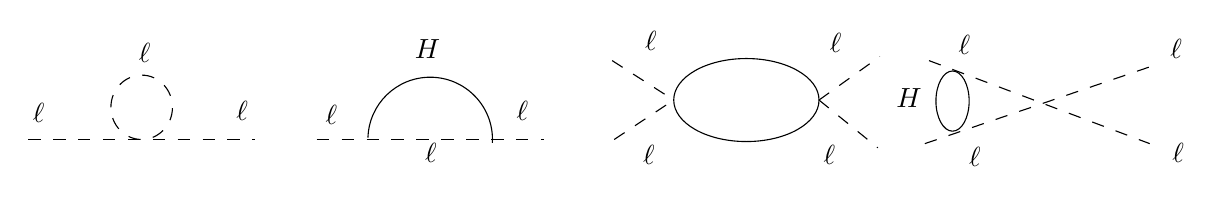
\begin{tikzpicture}[x=0.75pt,y=0.75pt,yscale=-1,xscale=1]
%uncomment if require: \path (0,300); %set diagram left start at 0, and has height of 300

%Straight Lines [id:da20190194107249004] 
\draw  [dash pattern={on 4.5pt off 4.5pt}]  (19,108) -- (128.33,108) ;
%Shape: Ellipse [id:dp4382337780369252] 
\draw  [dash pattern={on 4.5pt off 4.5pt}] (58.83,92.5) .. controls (58.83,83.94) and (65.47,77) .. (73.67,77) .. controls (81.86,77) and (88.5,83.94) .. (88.5,92.5) .. controls (88.5,101.06) and (81.86,108) .. (73.67,108) .. controls (65.47,108) and (58.83,101.06) .. (58.83,92.5) -- cycle ;
%Straight Lines [id:da7526492828725432] 
\draw  [dash pattern={on 4.5pt off 4.5pt}]  (158,108) -- (267.33,108) ;
%Shape: Arc [id:dp23282709893687115] 
\draw  [draw opacity=0] (182.68,107.1) .. controls (183.16,90.95) and (196.4,78) .. (212.67,78) .. controls (229.24,78) and (242.67,91.43) .. (242.67,108) .. controls (242.67,108.53) and (242.65,109.06) .. (242.63,109.59) -- (212.67,108) -- cycle ; \draw   (182.68,107.1) .. controls (183.16,90.95) and (196.4,78) .. (212.67,78) .. controls (229.24,78) and (242.67,91.43) .. (242.67,108) .. controls (242.67,108.53) and (242.65,109.06) .. (242.63,109.59) ;  
%Straight Lines [id:da1416926442165729] 
\draw  [dash pattern={on 4.5pt off 4.5pt}]  (300.33,70) -- (330,89) ;
%Shape: Ellipse [id:dp35200773626502946] 
\draw   (330,89) .. controls (330,77.95) and (345.67,69) .. (365,69) .. controls (384.33,69) and (400,77.95) .. (400,89) .. controls (400,100.05) and (384.33,109) .. (365,109) .. controls (345.67,109) and (330,100.05) .. (330,89) -- cycle ;
%Straight Lines [id:da18249428555639546] 
\draw  [dash pattern={on 4.5pt off 4.5pt}]  (301.33,108) -- (330,89) ;
%Straight Lines [id:da4536233532341827] 
\draw  [dash pattern={on 4.5pt off 4.5pt}]  (400,89) -- (429.33,68) ;
%Straight Lines [id:da15932171343342338] 
\draw  [dash pattern={on 4.5pt off 4.5pt}]  (400,89) -- (428.33,112) ;
%Straight Lines [id:da15701406098236637] 
\draw  [dash pattern={on 4.5pt off 4.5pt}]  (453,70) -- (559.33,110) ;
%Straight Lines [id:da43744840766161364] 
\draw  [dash pattern={on 4.5pt off 4.5pt}]  (451,110) -- (562.33,72) ;
%Shape: Ellipse [id:dp889615103333535] 
\draw   (456.33,89.5) .. controls (456.33,81.49) and (459.92,75) .. (464.33,75) .. controls (468.75,75) and (472.33,81.49) .. (472.33,89.5) .. controls (472.33,97.51) and (468.75,104) .. (464.33,104) .. controls (459.92,104) and (456.33,97.51) .. (456.33,89.5) -- cycle ;

% Text Node
\draw (20,89.4) node [anchor=north west][inner sep=0.75pt]    {$\ell $};
% Text Node
\draw (118,88.4) node [anchor=north west][inner sep=0.75pt]    {$\ell $};
% Text Node
\draw (71,60.4) node [anchor=north west][inner sep=0.75pt]    {$\ell $};
% Text Node
\draw (161,90.4) node [anchor=north west][inner sep=0.75pt]    {$\ell $};
% Text Node
\draw (209,108.4) node [anchor=north west][inner sep=0.75pt]    {$\ell $};
% Text Node
\draw (253,88.4) node [anchor=north west][inner sep=0.75pt]    {$\ell $};
% Text Node
\draw (204,58.4) node [anchor=north west][inner sep=0.75pt]    {$H$};
% Text Node
\draw (314,109.4) node [anchor=north west][inner sep=0.75pt]    {$\ell $};
% Text Node
\draw (315,54.4) node [anchor=north west][inner sep=0.75pt]    {$\ell $};
% Text Node
\draw (401,109.4) node [anchor=north west][inner sep=0.75pt]    {$\ell $};
% Text Node
\draw (404,55.4) node [anchor=north west][inner sep=0.75pt]    {$\ell $};
% Text Node
\draw (466,56.4) node [anchor=north west][inner sep=0.75pt]    {$\ell $};
% Text Node
\draw (471,110.4) node [anchor=north west][inner sep=0.75pt]    {$\ell $};
% Text Node
\draw (568,58.4) node [anchor=north west][inner sep=0.75pt]    {$\ell $};
% Text Node
\draw (569,108.4) node [anchor=north west][inner sep=0.75pt]    {$\ell $};
% Text Node
\draw (436,82.4) node [anchor=north west][inner sep=0.75pt]    {$H$};


\end{tikzpicture}
    \caption{Representative one-loop Feynman diagrams in the UV theory.}
    \label{fig:2}
\end{figure}

\noindent which involves divergent integrals of the type:
\begin{equation}
    \int \dfrac{d^4k}{k^2-M^2}
\end{equation}
However, experimental results give finite results of the observables. As we previously stated when we discussed the Wilsonian approach, we cannot use a momentum cut-off, so we need an alternative scheme to do the following\footnote{If the reader is not familiar with the following concepts, we highly encourage to read \cite{Olness_2011} first.}:
\begin{itemize}
    \item Perform those integrals and obtain finite results (i.e. \textit{regularize} the integrals). One possible scheme is to perform the integral in $4-2\epsilon$ dimensions, this is called \textit{dimensional regularization} \cite{Peskin:1995ev}.
    \item Find a way to fit the experimental values of the parameters with the values of the \textit{bare} parameters in (\ref{toymodellagrangianuv}) and (\ref{toymodelefflagrangian}). This leads to the idea we previously encountered: the couplings depend on the energy scale of our theory, following some differential equations called renormalization group equations. For instance, it could be proved that for a $\lambda_4$ term:
    \begin{equation}\label{runningcoupling}
        \lambda_4(E)=\dfrac{\lambda_4(\Lambda)}{1+\beta\lambda_4(\Lambda)\log(E/\Lambda)}
    \end{equation}
    which is closely related to the discussion we had about the instability of marginal operators. If $\beta>0$, then (\ref{runningcoupling}) is an increasing function around $E\to0$ so it becomes more relevant (it has a pole); but if $\beta<0$ the behavior is the opposite: it becomes irrelevant. Note that this is exactly what happens with the $\alpha_s$ of QCD and the $\alpha$ of QED, respectively.
\end{itemize}

With all of these in mind, we can proceed to apply the recipe we have developed in the previous section. Firstly, note that:
\begin{align}
    D_H&=-\partial^2-M^2\\
    D_l&=-\partial^2-m^2-\dfrac{\lambda_0}{2}\ell^2-\lambda_2H^2\\
    X_{lH}&=-\lambda^2\ell^2
\end{align}
and in particular:
\begin{equation}
     D_l(x,\partial_x+ip)=-p^2-\left(\partial^2+2ip_\mu\partial^\mu+\dfrac{\lambda_0}{2}\ell^2+\lambda_2H^2\right)
\end{equation}
With this particular arrangement, is easy to see that:
\begin{equation}
    D_l^{-1}=\dfrac{1}{p^2}\left( 1+\dfrac{m^2}{p^2}\right)+\dfrac{1}{p^4}\left(2ip_\mu\partial^\mu+\partial^2+\dfrac{\lambda_0}{2}\ell^2 \right)-4\dfrac{p_\mu p_\nu}{p^6}\partial^\mu\partial^\nu+\mathcal{O}(\zeta^{-6})
\end{equation}
thus, we only need to consider $n=1$ in the 1-loop effective Lagrangian (\ref{efflagrangian1loop}). Dropping the total derivative terms of the trace, we just need to compute:
\begin{equation}
    \mathcal{L}_{\text{eff}}^{\text{1-loop}}(\ell)=-\dfrac{i}{2}\int\dfrac{d^dp}{(2\pi)^d}\dfrac{U(x,\partial_x+ip)}{p^2-M^2}
\end{equation}
with:
\begin{equation}
    U(x,\partial_x+ip)=\dfrac{\lambda_1^2}{4}\ell^2\left[\dfrac{1}{p^2}\left(1+\dfrac{m^2}{p^2}\right)+\dfrac{1}{p^4}\left(2ip_\mu\partial^\mu+\partial^2+\dfrac{\lambda_0}{2}\ell^2 \right)  \right]\ell^2
\end{equation}
Note that if we fix $d=4$ we may obtain divergent terms, so we will use the dimensional regularization scheme. It is also convenient to use the following master integral formula \cite{Fuentes_Mart_n_2016}:
\begin{equation} \tag{20}
\begin{split}
\int \frac{d^d p}{(2\pi)^d} \frac{p_{\mu_1} \dots p_{\mu_{2k}}}{(p^2)^\alpha (p^2 - M^2)^\beta} 
&= \frac{(-1)^{\alpha+\beta+k} i}{(4\pi)^{\frac{d}{2}}} 
\frac{\Gamma \left( \frac{d}{2} + k - \alpha \right) \Gamma \left( -\frac{d}{2} - k + \alpha + \beta \right)}{\Gamma(\beta) \Gamma \left( \frac{d}{2} + k \right)} \\
&\quad \times \frac{g_{\mu_1 \dots \mu_{2k}}}{2^k} M^{d+2k-2\alpha-2\beta} \,,
\end{split}
\end{equation}
where $g_{\mu_1 \dots \mu_{2k}}$ is the totally symmetric tensor with $2k$ indices constructed from $g_{\mu\nu}$ tensors. And also that (see section 7.5 of \cite{Peskin:1995ev}):
\begin{equation}
    \Gamma(\epsilon)=\dfrac{1}{\epsilon}-\gamma+\mathcal{O}(\epsilon)\quad,\quad  \Gamma(1-\epsilon)\approx1 \quad,\quad \Gamma(2-\epsilon)=(1-\epsilon)\Gamma(1-\epsilon)\approx1-\epsilon
\end{equation}
The possible remaining ${1}/{\epsilon}-\gamma$ terms can be dropped assuming that they are absorbed in the bare coupling constants. Hence, we finally obtain:
\begin{equation}\label{1looplagrangianaftercuentas}
    \mathcal{L}_{\text{eff}}^{\text{1-loop}}(\ell)=\dfrac{\lambda_1^2}{16(16\pi^2)}\left[2\left(1+\dfrac{m^2}{M^2}\right)\ell^4-\dfrac{1}{M^2}\ell^2\partial^2\ell^2+\dfrac{\lambda_0}{M^2}\ell^6  \right]+\mathcal{O}(1/M^4)
\end{equation}
which is a local and well-behaved in the limit $M\to \infty$ Lagrangian. Notice that the differential operator can be rearranged as follows:
\begin{equation}
    \ell(\partial\ell)^2=-\dfrac{1}{3}\ell^3\partial^2\ell+\partial(\ell^3\partial\ell)
\end{equation}
so the second term of the right hand side can be dropped from the Lagrangian (\ref{1looplagrangianaftercuentas}) and the first term can be rewritten in terms of $\ell^4$ and $\ell^6$ as we previously did. As we could expect from the initial discussion, the 1-loop effective Lagrangian modifies the couplings $C_4$ and $C_6$.
\section{Conclusions}
In this work, we have presented the fundamental concepts of Effective Field Theories, emphasizing their power in simplifying the description of physical systems by focusing on the relevant degrees of freedom at a given energy scale. We also introduced the Wilsonian effective action formalism, demonstrating how heavy degrees of freedom can be integrated out to generate a tower of local operators, as it was explicitly illustrated through a toy model of two scalar fields, where we performed matching at both tree-level and one-loop order.

Throughout this text we focused only on the \textit{top-down} approach to EFTs, where the full high-energy (UV) theory is known. By integrating out the heavy field, we derived the low-energy coefficients explicitly in terms of the couplings of the more fundamental theory. Conversely, the other approach is called \textit{the bottom-up} and it is used when the UV theory is unknown. In this scenario, one constructs the most general Lagrangian consistent with the assumed symmetries of the light degrees of freedom and the Wilson coefficients are then treated as free parameters to be determined by experiments (the most illustrative example is the Standard Model Effective Field Theory or SMEFT \cite{manohar2018introductioneffectivefieldtheories, Burgess_2007, Falkowski,Fuentes_Mart_n_2016}). 

As our approach for 1-loop calculations was not based in Feynman diagrams, we did not explain the \textit{power counting rules} \cite{Burgess_2007}, which link the number of loops and vertices in a graph with the ratio $m/M$. Furthermore, our discussion was limited to scalar fields as the inclusion of fermion field introduces additional complexity. 

Finally, we briefly encountered the concept of field redefinitions when simplifying the dimension-six operators. In general, operators that vanish due to the equations of motion are redundant and can be removed by an appropriate field redefinition. This is a crucial tool in EFTs, as it allows us to reduce the basis of operators to a minimal independent set and we do not overcount the physical parameters of the theory.
\section*{Use of AI}
No AI was used during the development of these notes. The diagrams were done using the \href{https://tikz.net/}{Tikz} package and the references were hand-picked with the help of the professor Verónica Sanz. All of the possible typos (there surely are a few) are exclusively my fault.

\appendix

\newpage

\printbibliography

\end{document}
